\documentclass{chemlab}
\usepackage{hyperref}
\usepackage{fancyhdr}
\usepackage{graphicx}
\usepackage{amssymb}
\usepackage{longtable}
\usepackage{booktabs}
\usepackage{gensymb}
\usepackage{csvsimple}
\usepackage{booktabs}
\usepackage{longtable}
\usepackage{array}
\usepackage{multirow}
\usepackage{wrapfig}
\usepackage{float}
\usepackage{colortbl}
\usepackage{pdflscape}
\usepackage{tabu}
\usepackage{threeparttable}
\usepackage{threeparttablex}
\usepackage[normalem]{ulem}
\usepackage{makecell}
\usepackage{xcolor}

\fancyhead[L,C, R]{}
\fancyhead[C]{Edouard Des Parois Perrault}
\fancyfoot[C]{
\includegraphics[scale=0.15]{template_images/edouard-seal.png}}
\fancyfoot[R]{\thepage}
\renewcommand{\headrulewidth}{0.4pt}
\renewcommand{\footrulewidth}{2pt}
\renewcommand{\headheight}{15pt}
\renewcommand{\footskip}{80pt}

\providecommand{\tightlist}{%
  \setlength{\itemsep}{0pt}\setlength{\parskip}{0pt}}

\pagestyle{fancy}

\title{Coefficient of Friction Lab Report}
\subject{Physics}
\teacher{Shawn Weiland}
\author{Edouard Des Parois Perrault}
\date{18/02/2021}
\begin{document}
    \maketitle
        \tableofcontents
        \hypertarget{calculating-error-bars}{%
\section{\texorpdfstring{Calculating Error Bars
\label{sec:err}}{Calculating Error Bars }}\label{calculating-error-bars}}

The instrumental error was calculated based on the instrument. For
analog instruments, it is equal to half of the smallest graduation. The
procedural error was calculated using the formula in Equation
\eqref{eqn:error}.

\begin{equation}
  E_{\text{procedural}} = \frac{\text{max} - \text{min}}{2} \label{eqn:error}
\end{equation}

As an example, I will calculate the procedural error for the first
trial, which was for a mass of 187.60 grams. The results are in Table
\ref{tab:trials}.

\begin{table}[H]

\caption{\label{tab:trials}Data for a mass of 187.60 grams}
\centering
\begin{tabular}[t]{rr}
\toprule
Trial & Force\\
\midrule
\cellcolor{gray!6}{1} & \cellcolor{gray!6}{0.15}\\
2 & 0.10\\
\cellcolor{gray!6}{3} & \cellcolor{gray!6}{0.05}\\
\bottomrule
\end{tabular}
\end{table}

\begin{eqnarray}
  E_{\text{procedural}} & = & \frac{\text{max} - \text{min}}{2} \\
                        & = & \frac{0.15-0.05}{2} \\
                        & = & 0.05 
\end{eqnarray}

When calculating the error bars, the largest of the two errors was used.
A complete rundown of all error calculations is on Table
\ref{tab:error-bars}.

\begin{table}

\caption{\label{tab:error-bars}Error Bar Values}
\centering
\begin{tabular}[t]{rrr}
\toprule
Instrumental Error & Procedural Error & Largest\\
\midrule
\cellcolor{gray!6}{0.03} & \cellcolor{gray!6}{0.05} & \cellcolor{gray!6}{\vphantom{4} 0.05}\\
0.03 & 0.05 & \vphantom{3} 0.05\\
\cellcolor{gray!6}{0.03} & \cellcolor{gray!6}{0.05} & \cellcolor{gray!6}{\vphantom{2} 0.05}\\
0.03 & 0.03 & 0.03\\
\cellcolor{gray!6}{0.03} & \cellcolor{gray!6}{0.05} & \cellcolor{gray!6}{\vphantom{1} 0.05}\\
\addlinespace
0.03 & 0.05 & 0.05\\
\cellcolor{gray!6}{0.10} & \cellcolor{gray!6}{0.10} & \cellcolor{gray!6}{\vphantom{1} 0.10}\\
0.10 & 0.10 & 0.10\\
\bottomrule
\end{tabular}
\end{table}

\hypertarget{applied-force-values}{%
\section{\texorpdfstring{Applied Force Values
\label{sec:applied-force}}{Applied Force Values }}\label{applied-force-values}}

The applied force values for each trial were averaged out. The average
values can be found in Table \ref{tab:final-data}. Note that the normal
force was calculated in Section \ref{sec:normal-force} For the example
below, I will be using data from Table \ref{tab:trials}.

\begin{eqnarray}
  \text{avg} & = & \frac{0.15 + 0.10 + 0.05}{3} \\
             & = & 0.1
\end{eqnarray}

\begin{table}

\caption{\label{tab:final-data}Normal Force versus Applied Force}
\centering
\begin{tabular}[t]{rr}
\toprule
Normal Force (N) & Applied Force (N)\\
\midrule
\cellcolor{gray!6}{1.84} & \cellcolor{gray!6}{1.00}\\
3.80 & 0.50\\
\cellcolor{gray!6}{5.76} & \cellcolor{gray!6}{0.90}\\
7.72 & 1.42\\
\cellcolor{gray!6}{9.68} & \cellcolor{gray!6}{1.85}\\
\addlinespace
11.64 & 2.35\\
\cellcolor{gray!6}{13.60} & \cellcolor{gray!6}{2.60}\\
18.01 & 4.27\\
\bottomrule
\end{tabular}
\end{table}

\hypertarget{determine-the-normal-force}{%
\section{\texorpdfstring{Determine the Normal Force
\label{sec:normal-force}}{Determine the Normal Force }}\label{determine-the-normal-force}}

The weight of the object can be calculated using the mass of the object
in kilograms, \(m\), as well as the gravitational acceleration of Earth,
\(a\), using Equation \eqref{eqn:weight}.

\begin{equation}
  W = ma \label{eqn:weight}
\end{equation}

The following is a sample calculation for the weight of the object. Note
that the mass of the object is in grams, so it must be converted.

\begin{eqnarray}
  W & = & ma \\
    & = & \frac{187.6}{1000} \cdot 9.81 \\
    & \approx & 1.84
\end{eqnarray}

Note that the normal force is equivalent to the weight. The reason for
this is that normal force is defined as being the force that is
perpendicular to the object and pushes back on it to prevent it from
falling. Because the object is still on the table, the normal force must
be equal to its weight. If the normal force was greater than its weight,
it would levitate, and if it was less than its weight, it would be
falling.

The weight (and therefore the normal force) for each object is compiled
in Table \ref{tab:normal-force}.

\begin{table}

\caption{\label{tab:normal-force}Calculating Weight with Mass}
\centering
\begin{tabular}[t]{cc}
\toprule
Mass (g) & Weight (N)\\
\midrule
\cellcolor{gray!6}{187.6} & \cellcolor{gray!6}{1.83848}\\
387.6 & 3.79848\\
\cellcolor{gray!6}{587.6} & \cellcolor{gray!6}{5.75848}\\
787.6 & 7.71848\\
\cellcolor{gray!6}{987.6} & \cellcolor{gray!6}{9.67848}\\
\addlinespace
1187.6 & 11.63848\\
\cellcolor{gray!6}{1387.6} & \cellcolor{gray!6}{13.59848}\\
1837.6 & 18.00848\\
\bottomrule
\end{tabular}
\end{table}

\hypertarget{maximum-static-friction}{%
\section{Maximum Static Friction}\label{maximum-static-friction}}

The maximum static friction force was calculated by taking the average
value of all trials (as shown in Section \ref{sec:applied-force}) and
adding the error (as shown in Section \ref{sec:err}). As an example,
using the data from Table \ref{tab:trials}:

\begin{eqnarray}
  \text{Max Force} & = & 1 + 0.05 \\
                   & = & 1.05
\end{eqnarray}

The total forces can be found in Table \ref{tab:max-fric}.

\begin{table}[H]

\caption{\label{tab:max-fric}Maximum Static Friction}
\centering
\begin{tabular}[t]{c|c}
\hline
Normal Force (N) & Maximum Force of Friction (N)\\
\hline
\cellcolor{gray!6}{1.84} & \cellcolor{gray!6}{1.05}\\
\hline
3.80 & 0.55\\
\hline
\cellcolor{gray!6}{5.76} & \cellcolor{gray!6}{0.95}\\
\hline
7.72 & 1.45\\
\hline
\cellcolor{gray!6}{9.68} & \cellcolor{gray!6}{1.90}\\
\hline
11.64 & 2.40\\
\hline
\cellcolor{gray!6}{13.60} & \cellcolor{gray!6}{2.70}\\
\hline
18.01 & 4.37\\
\hline
\end{tabular}
\end{table}

\hypertarget{draw-a-free-body-diagram-of-the-situation}{%
\section{Draw a Free Body Diagram of the
Situation}\label{draw-a-free-body-diagram-of-the-situation}}

The free-body diagram of the object is in Figure \ref{fig:object}. The
free body diagram of the table is in Figure \ref{fig:table}.

\begin{figure}[H]

{\centering 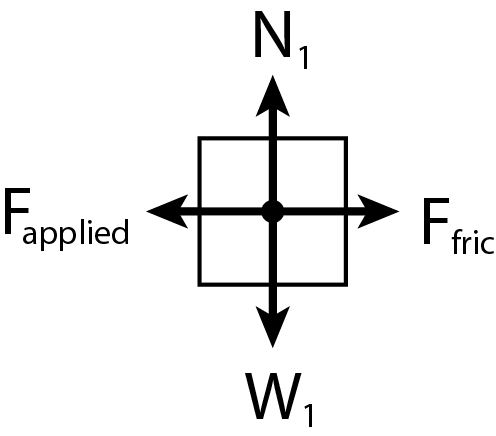
\includegraphics[height=10cm]{./images/object-diagram} 

}

\caption{Free Body Diagram of Object}\label{fig:object}
\end{figure}

\begin{figure}[H]

{\centering 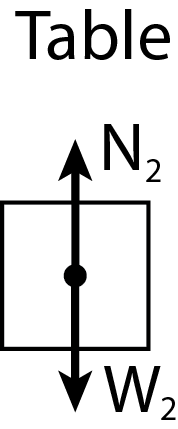
\includegraphics[height=10cm]{./images/table-diagram} 

}

\caption{Free Body Diagram of Table}\label{fig:table}
\end{figure}

\hypertarget{graph}{%
\section{Graph}\label{graph}}

The graph of this experiment is in Figure \ref{fig:graph}.

\begin{figure}[H]

{\centering 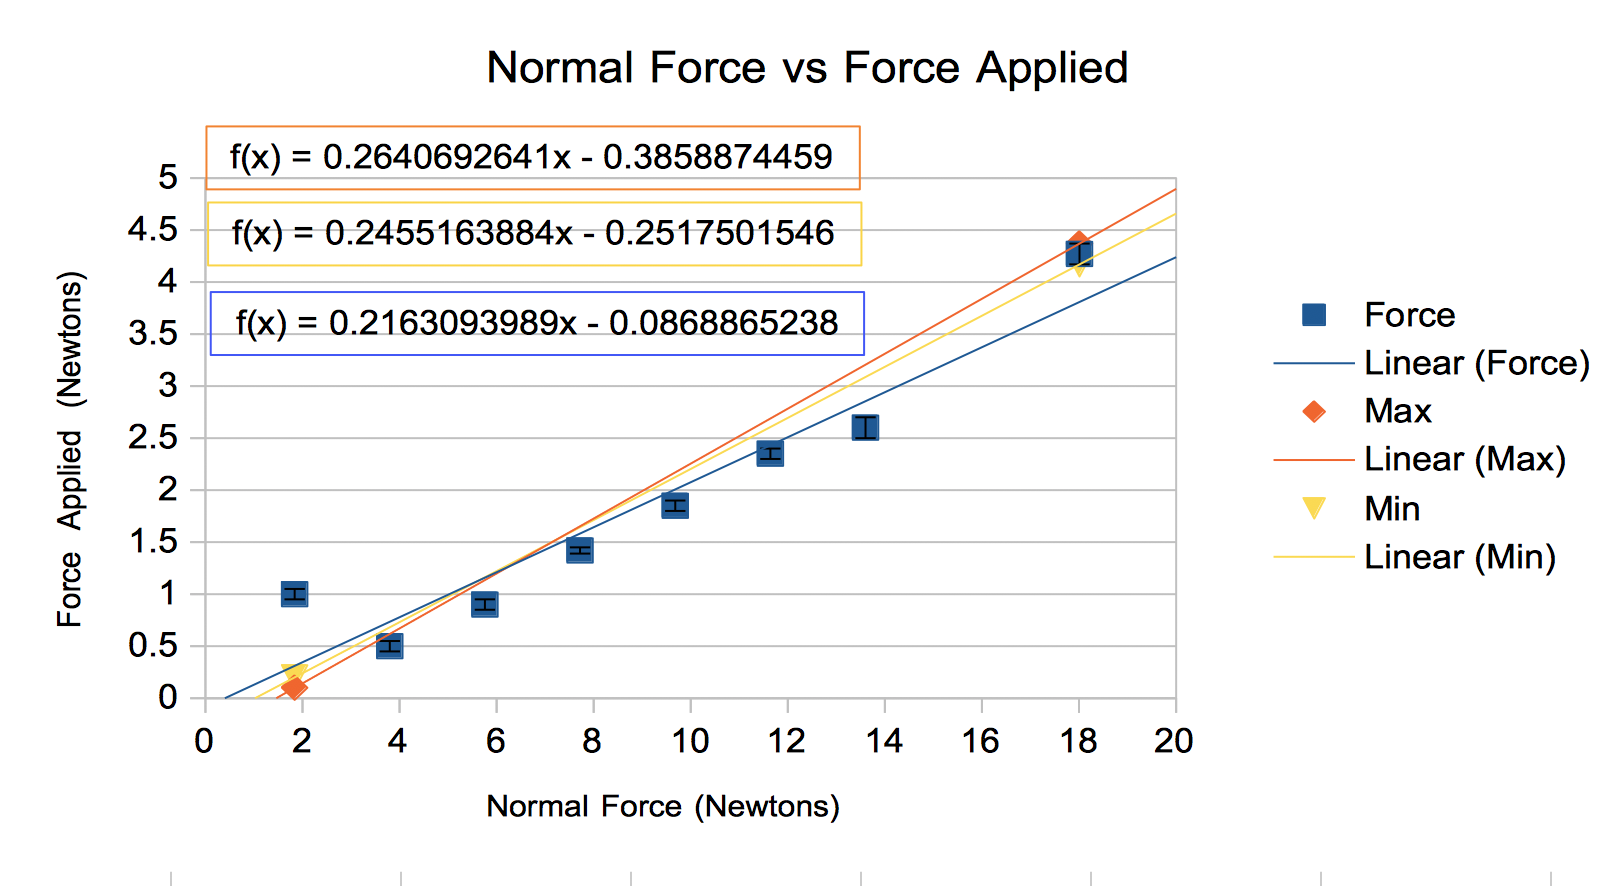
\includegraphics[height=5cm]{./images/graph} 

}

\caption{Normal Force vs Force Applied}\label{fig:graph}
\end{figure}

The slopes are in the graph. For reference, the slope of the line of
best fit is 0.216, the slope of the minimum trend line is 0.246, and the
slope of the maximum trend line is 0.264. Note that the slope of the
line of best fit is effectively below the slope of the minimum trend
line; this is due to the fact that the points are very spread out.
\end{document}